\documentclass{article}
\usepackage[utf8]{inputenc}
\usepackage{listings}
\usepackage{epsfig} %% for loading postscript figures
\usepackage{indentfirst}

\usepackage{bm}
\usepackage{amsfonts}
\usepackage{amsmath}

\usepackage{hyperref}
\title{VAE}
\author{Caoyuan}
\date{September 2017}

\begin{document}
\bibliographystyle{plain}

\maketitle
\section{Notes from others}
Notes from \href{https://zhuanlan.zhihu.com/p/27197322}{HERE}


Background: 


1. Intractability. A. Integral of the marginal likelihood $p_{\theta}(x) = \int p_\theta(z)p_\theta(x|z)dz$ is intractable, B. True posterior density $p_{\theta}(z|x)=p_\theta(z|x) =p_\theta(x|z)p_\theta(z)/p_\theta(x)$ is intractable, so EM can not be used. C. Required integrals for any reasonable mean-field VB algorithm are also intractable.


2. Large dataset, using Monte Carlo EM, cost too much time


Variational Inference Summary:


use $q_\phi(z|x)$ to approximate $p_\theta(z|x)$, minimize KL divergence between them.
\begin{figure}
\centering
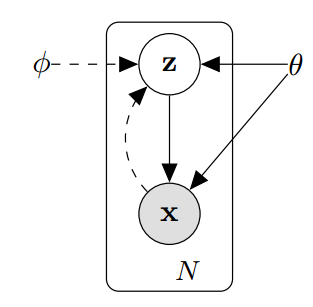
\includegraphics[width = .5\textwidth]{vae.png}
\caption{graph}
\label{fig:model}
\end{figure}

\begin{equation}
\begin{split}
&D_{KL}[q_{\phi}(z)||p_\theta(z|x)] = \int q_\phi (z)log\frac{q_\phi (z)}{p_\theta(z|x)}dz = \int q_\phi (z)log\frac{q_\phi (z) p_\theta(x)}{p_\theta(x,z)}dz\\
&=\int q_\phi(z)log \frac{q_\phi (z)}{p_\theta(x,z)}dz + \int q_\phi(z)log\ p_\theta(x)dz=\int q_\phi (z)(logq_\phi (z) - log\ p_\theta(x,z))dz + logp_\theta(x)\\
&=-(E_{q_{\phi}(z)}log\ p_\theta(x,z) - E_{q_{\phi}(z)}log\ q_\phi(z))+ logp_\theta(x)\\
\end{split}
\end{equation}

The first item is the negative ELBO(Evidence lower Bound)

According to which we can get the equation of the paper:
$logp_\theta(x^{(i)}) = D_{KL}(q_\phi (z|x)^{(i)}||p_\theta(z|x^{(i)}))+ L(\theta,\phi;x^{(i)})$


Where $p(x)$ is fixed, $log\ p(x_\theta^{(i)})$ is constant, to minimize the first term of RHS, equals to maximize the second term.


So that given $x$, $q_\phi(z|x)$ can get the distribution of $z$, it's called ENCODER, also $p_\theta(x|z)$ is called decoder.


Another way to get the ELOB:
\begin{equation}
log\ p(x) = log\int\ p(z,x)dz=log\int q(z|x)(\frac{p(z,x)}{q(z|x)})dz \geq \int q(z|x)log(\frac{p(z,x)}{q(z|x)})dz = L(\theta, \phi;x)
\end{equation}

The second term can be seen as:
\begin{equation}
\begin{split}
&L(\theta, \phi;x) = -\int q_\phi(z|x) log(\frac{q_\phi(z|x)}{p_{\theta}(z)*p_{\theta}(x|z)})dz = \int q_\phi(z|x) log\ p_{\theta}(x|z))dz - D_{KL}(q_\phi(z|x)||p_\theta(z))\\
&=E_{q_\phi(z|x)}[log\ p_\theta(x|z)] - D_{KL}(q_\phi(z|x)||p_\theta(z))\\
\end{split}
\end{equation}


The first term can be seen as \underline{reconstruction error}, the second term can be seen as \underline{regularization term}.


Since $\nabla_\phi E_{q_\phi(z|x)}[log\ p_\theta(x|z)]$ is intractable, we use Monte Carlo gradient estimator to estimate the value. Set $f(z) = log\ p(x|z)$

\begin{equation}
\begin{split}
&\nabla_\phi E_{q_\phi(z|x)}[f(z)] = \nabla_\phi \int q_{\phi}(z)f(z)dz =  \int q_{\phi}(z)f(z)(\frac{\nabla_\phi q_{\phi}(z)}{q_{\phi}(z)})dz = \int q_{\phi}(z)f(z)\nabla_\phi log\ q_{\phi}(z) dz\\ 
&= E_{q_\phi(z|x)}[f(z)\nabla_\phi log\ q_{\phi}(z)] \approx \frac{1}{L}\sum_{l=1}^{L} f(z)\nabla_\phi log\ q_{\phi}(z^{l}) where\ z^{(l)} \sim q_\phi(z)\\
\end{split}
\end{equation}


Here, according the paper section 2.2, subscript shall be $\nabla_{q_\phi(z)}$, \underline{\textbf{What's the difference?}}

Which means to sample $L$ samples from distribution $q_\phi(z)$ as the Expectation of $f(z)\nabla_\phi log\ q_{\phi}(z)$, as $E_{q_\phi(z)}[f(z)\nabla_\phi log\ q_{\phi}(z)]$


Now the object function becomes:
\begin{equation}
\begin{split}
&L(\theta, \phi, x^{(i)}) =- D_{KL}(q_\phi(z|x^{(i)})||p_\theta(z)) + E_{q_\phi(z|x^{(i)})}[log\ p_\theta(x^{(i)}|z)] \\
&Monte\ Carlo\ Gradient\ Estimator\\
&\hat{L}^A(\theta, \phi, x^{(i)}) \approx L(\theta, \phi, x^{(i)})\ \ ??\\
&\hat{L}^A(\theta, \phi, x^{(i)}) = - D_{KL}(q_\phi(z|x^{(i)})||p_\theta(z)) + \frac{1}{L}\sum_{l=1}^{L} log\ p_\theta(x^{(i)}|z^{(i,l)})]\\
&\hat{L}^A(\theta, \phi, x^{(i)}) = \frac{1}{L}\sum^L_{l=1}\ log\ p_\theta(x^{(i)},z^{(i,l)}) - log\ q_\phi (z^{i,l}|x^{(i)})\\
&where\ z^{(i, l)}=g_\phi(\epsilon^{(i,l)}, x^{(i)})\ and\ \epsilon^{l} \sim p(\epsilon)
\end{split}
\end{equation}


The disadvantage of this method is the variance is large, it's not practical. So use reparameterization trick, sampling becomes:
\begin{equation}
\begin{split}
&z \sim q_\phi(z|x)\\
&auxiliary\ variable\\
&\epsilon \sim p(\epsilon)\\
&determinstic\ variable\\
&z = g_\phi(\epsilon, x)\\
&Example:\\
&z \sim p(z|x) = N(\mu, \sigma^2)\ \ \epsilon \sim N(0,1)\ z=\mu +\sigma \epsilon
\end{split}
\end{equation}



\section{Notes}
There are two downsides of GAN. first, if you want to generate a picture with specific features, there's no way of determining which initial noise value would produce that picture, other than searching over the entire distribution. Second, a generative adversarial model only discriminates between "real" and "fake" images. There's no constraints that an image of a cat has to look like a cat. This leads to results where there's no actual object in a generated image, but the style just looks like picture.


Soultion: Add a constraint on the encoding network, forces it to generate latent vectors that roughly follow a unit gaussian distribution. This constrain separates a variational autoencoder from a standard one. Then we can sample a latent vector from the unit gaussian and pass it to the decoder. There's a trade off between how accurate our network can be and how close its latent variable can match the unit gaussian distribution. The network decide this itself. sum up two separate losses: generative loss(suqared error that measures how accurately the network reconstruncted the images) and latent loss(KL divergence that measureshow closely the latent variables match a unit gaussian).


Reparameterization trick: Instead of the encoder generating a vector of real values, it generate a vector of means and a vector of standard deviations.


The greater standard deviation on the noise added, the less information we can pass using that one variable.


Formalize: we get examples $X$ distributed according to some unknown distribution $P_{gt}(X)$, and the goal is to learn a model $P$ which we can sample from, such that $P$ is as similar as possible to $P_{gt}$.

Drawbacks: 1) Strong assumptions about the structure in the data. 2) they might make severe approximations, leading to suboptimal models. 3) They might rely on computationally expensive inference procedures like MCMC.


The key idea behind the variational autoencoder is to attempt to sample values of z that are likely to have produced X, and compute P(X) just from those.

$Q$ is "encoding" $X$ to $z$, and $P$ is "decoding" $z$ to $X$.




\begin{equation}
\begin{split}
\int q_\theta(\boldsymbol{z})log\ p(\boldsymbol{z})d\boldsymbol{z} &= \int N(\boldsymbol{z};\boldsymbol{\mu}, \boldsymbol{\sigma}^2)log\ N(\boldsymbol{z};\boldsymbol{0},\boldsymbol{I})d\boldsymbol{z}\\
&=\int N(\boldsymbol{z};\boldsymbol{\mu}, \boldsymbol{\sigma}^2)\{-\frac{J}{2}log 2\pi -\frac{1}{2} \sum_{j=1}^J z_j^2\}d\boldsymbol{z}\\
&=-\frac{J}{2}log 2\pi -\int N(\boldsymbol{z};\boldsymbol{\mu}, \boldsymbol{\sigma}^2)\frac{1}{2} \sum_{j=1}^J z_j^2\\
&=-\frac{J}{2}log 2\pi -\frac{1}{2}\int_{z_1} \int_{z_2}\dots\int_{z_J} N(\boldsymbol{z};\boldsymbol{\mu}, \boldsymbol{\sigma}^2) (z_1^2+z_2^2+\dots+z_j^2)dz_1dz_2\dots dz_J\\
&=-\frac{J}{2}log 2\pi -\frac{1}{2}(\int_{z_1} N(\boldsymbol{z};\boldsymbol{\mu}, \boldsymbol{\sigma}^2) z_1^2d\boldsymbol{z}+\dots \int_{z_J} N(\boldsymbol{z};\boldsymbol{\mu}, \boldsymbol{\sigma}^2) z_J^2d\boldsymbol{z})\\
&=-\frac{J}{2} log(2\pi)-\frac{1}{2}\sum^J_{j=1}(\mu_j^2+\sigma_j^2)
\end{split}
\end{equation}

\begin{equation}
\begin{split}
\int q_\theta(\boldsymbol{z})log\ q_\theta(\boldsymbol{z})d\boldsymbol{z} &= \int N(\boldsymbol{z};\boldsymbol{\mu}, \boldsymbol{\sigma}^2)log\ N(\boldsymbol{z};\boldsymbol{\mu}, \boldsymbol{\sigma}^2)d\boldsymbol{z}\\
&=\int N(\boldsymbol{z};\boldsymbol{\mu}, \boldsymbol{\sigma}^2) \sum_{j=1}^J(-\frac{1}{2}log(2\pi \sigma_j^2)-  \frac{1}{2\sigma_j^2}(z_j-\mu_j)^2) d\boldsymbol{z}\\
&=-\frac{J}{2}log(2\pi) - \frac{1}{2}\sum_{j=1}^J log(\sigma_j^2)+ \int N(z_1;\mu_1, \sigma_1^2) (-  \frac{1}{2\sigma_1^2}(z_1-\mu_j)^2) dz_1 + \dots \\
&+ \int N(z_J;\mu_J, \sigma_J^2) (-  \frac{1}{2\sigma_J^2}(z_J-\mu_J)^2) dz_J\\
&=-\frac{J}{2}log(2\pi) - \frac{1}{2}\sum_{j=1}^J log(\sigma_j^2)+ \sum_{j=1}^J\int N(z_j;\mu_j, \sigma_j^2) (-\frac{1}{2\sigma_j^2}(z_j-\mu_j)^2)dz_j\\
&=-\frac{J}{2}log(2\pi) - \frac{1}{2}\sum_{j=1}^J log(\sigma_j^2)+ \sum_{j=1}^J\int N(z_j;\mu_j, \sigma_j^2) (-\frac{z_j^2-2\mu_j^2+\mu_j^2}{2\sigma_j^2})dz_j\\
&=-\frac{J}{2}log(2\pi) - \frac{1}{2}\sum_{j=1}^J log(\sigma_j^2)+ \sum_{j=1}^J-\frac{\mu^2+\sigma_j^2-2\mu_j+\mu_j^2}{2\sigma_j^2}\\
&=-\frac{J}{2}log(2\pi) - \frac{1}{2}\sum_{j=1}^J(1+log\ \sigma_j^2)\\
\end{split}
\end{equation}


Therfore:
\begin{equation}
\begin{split}
-D_{KL}(q_{\boldsymbol{\phi}}(\boldsymbol{z})||p_{\boldsymbol{\theta}}(\boldsymbol{z})) &= \int q_{\boldsymbol{\theta}}(\boldsymbol{z})(log\ p_{\boldsymbol{\theta}}(\boldsymbol{z}) - log\ q_{\boldsymbol{\theta}}(\boldsymbol{z}))\\
&=\frac{1}{2}\sum_{j=1}^J(1+log((\sigma_j)^2) - (\mu_j)^2 - (\sigma_j)^2)
\end{split}
\end{equation}

Here, why the parameter is changed from $\phi$ to $\theta$





\section{Questions}
One-shot approximate inference

VAEs are based on \underline{"Minimum description length"} coding model


$L(q,x) = \int q(h|x)log\ p(x|h)dh - D(q(h|x)||p(h))$
First iterm is called \underline{reconstruncion error}, why? What's the physis meaning of  


Now we can apply this same logic to the latent variable passed between the encoder and decoder. The more efficiently we can encode the original image, the \underline{\textbf{higher}} we can raise the standard deviation on our gaussian until it reaches one.


//$P(X|z;\theta) = N(X|f(z;\theta),\sigma^2 * I)$, but there is no $\sigma$ on the graph?

\begin{figure}
\centering
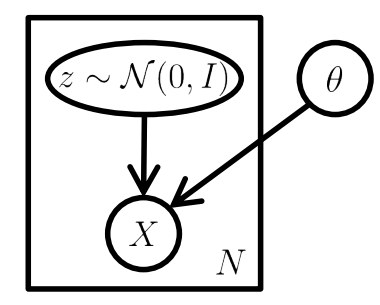
\includegraphics[width = .5\textwidth]{model.png}
\caption{graph}
\label{fig:data}
\end{figure}


isotropic Gaussian?


Figure 3 of tutorial on VAE, very small different between b and c


The whole equation we want to optimize is:
\begin{equation}
E_{X\sim D}[log\ P(X)- D[Q(z|X)||P(z|X)]] = E_{X\sim D}[E_{z\sim Q}[log\ P(X|z) - D[Q(z|X)||P(z)]].
\end{equation}

The gradient symbol can be moved into the expectations?(Why, Black box ?)


The equation we actually take the gradient of is:
\begin{equation}
E_{X\sim D}[E_{\epsilon \sim N(0, I)}[log\ P(X|z=\mu(X)+\Sigma^{1/2}(X)*\epsilon)]- D[Q(z|X)||P(z)]]
\end{equation}
What's the Second expection with respect to? Why it's not respect to $Q(x)$ anymore


"Reparameterization trick" only works if we can sample from $Q(z|X)$ by evaluating a function $h(\eta, X)$, where $\eta$ is noise from a distribution that is not learned.


Sampling $z$ from $Q$ gives an estimator for the expectation which generally converges much faster than sampling $z$ from $N(0,1)$ as discussed in section (P12 of tutorial) 2. Why?


$p_{\theta}(z)$ and $p_{\theta}(x|z)$ use the same parameter? 


// The usual MonteCarlo gradient estimator for this type of problem is: $\nabla_{\phi}E_{q_{\phi}(z)}[f(z)] = E_{q_{\phi}(z)}[f(z)\nabla_{q_{\phi}(z)}log\ q_{\phi}(z)]$,(Solved according to Black box or above equations)

\begin{equation}
E_{q_{\phi}(z|x^{(i)})}[f(z)] = E_{p(\epsilon)}[f(g_{\phi}(\epsilon, x^{(i)}))],\ where\ \epsilon^{l} \sim p(\epsilon)
\end{equation}


Given the deterministic mapping $z = g_{\phi}(\epsilon, x)$ we know that $q_{\phi}\prod_idz_i = p(\epsilon)\prod_id\epsilon_i$. why?


Used Gaussian as the form of $q(z|x)$ and $p(x|z)$, why?


According to \underline{Black box VI}, $\nabla_{\lambda}[log\ p(x,z)] = 0$, but according to \underline{VAE}, $\nabla_{\phi}E_{q(z|x)}[log\ p_{\theta}(x|z)]$ is intractable.


Both used the trick $\nabla_{\phi}log\ q_{\phi}(z) = \frac{\nabla_{\phi}q_{\phi}(z)}{q_{\phi}(z)}$

Is both method solved the problem of huge variance?

Is the function of reparameterization trick for \underline{reduce variance} or to make the equation continus?(Make sampling as input then we can get the derivative)

Why to make $q_\phi(z|x)$ as close to Gaussian distribution as possible?


Recognition model?


\begin{equation}
\begin{split}
&\boldsymbol{\varphi}_{k=1\dots K} \sim Dirichlet_V(\boldsymbol{\beta}) \\
&\boldsymbol{\theta}_{d=1\dots M} \sim Dirichlet_K(\boldsymbol{\alpha})\\
&z_{d=1\dots M, w= 1\dots N_d} \sim Categorical_K(\boldsymbol{\theta}_d)\\
&w_{d=1\dots M, w= 1\dots N_d} \sim Categorical_V(\boldsymbol{\varphi}_{z_{dw}})\\
\end{split}
\end{equation}

\begin{figure}
\centering
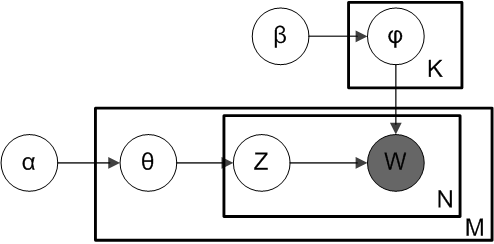
\includegraphics[width = .5\textwidth]{lda.png}
\caption{graph}
\label{fig:lda}
\end{figure}

Inference of LDA refer to \href{https://en.wikipedia.org/wiki/Latent_Dirichlet_allocation}{WIKI}.
\section{future work}

Variational Bayesian Inference with Stochastic Search


Deep latent dirichlet allocation with topic-layer-adaptive stochastic gradient riemannian mcmc
\bibliography{bibfile}
\end{document}